\begin{figure}[H]
\centering

\begin{subfigure}{.4\textwidth}
  \centering
  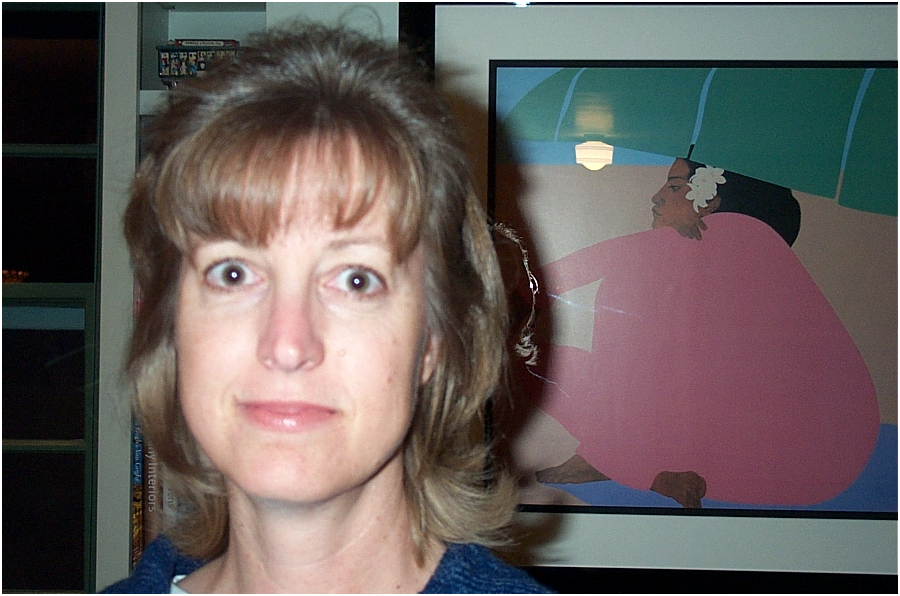
\includegraphics[width=0.95\textwidth]{img/fd/Original.png}
  \caption{}
  % \label{fig:sub1}
\end{subfigure}%

\begin{subfigure}{.24\textwidth}
  \centering
  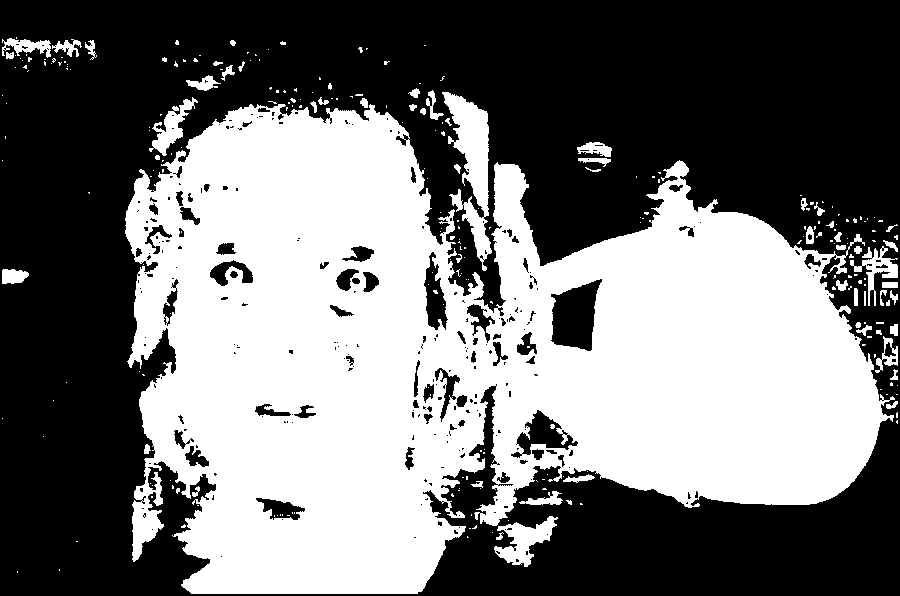
\includegraphics[width=0.95\textwidth]{img/fd/EstimatedSkinMask.png}
  \caption{}
  % \label{fig:sub1}
\end{subfigure}%
\begin{subfigure}{.24\textwidth}
  \centering
  % 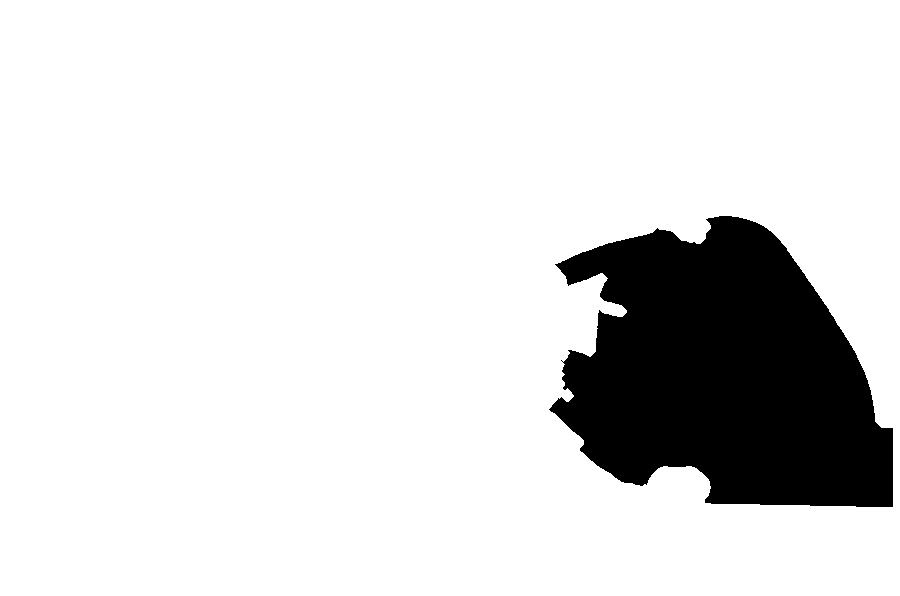
\includegraphics[width=0.95\textwidth]{img/fd/ForeGroundMask.png}
  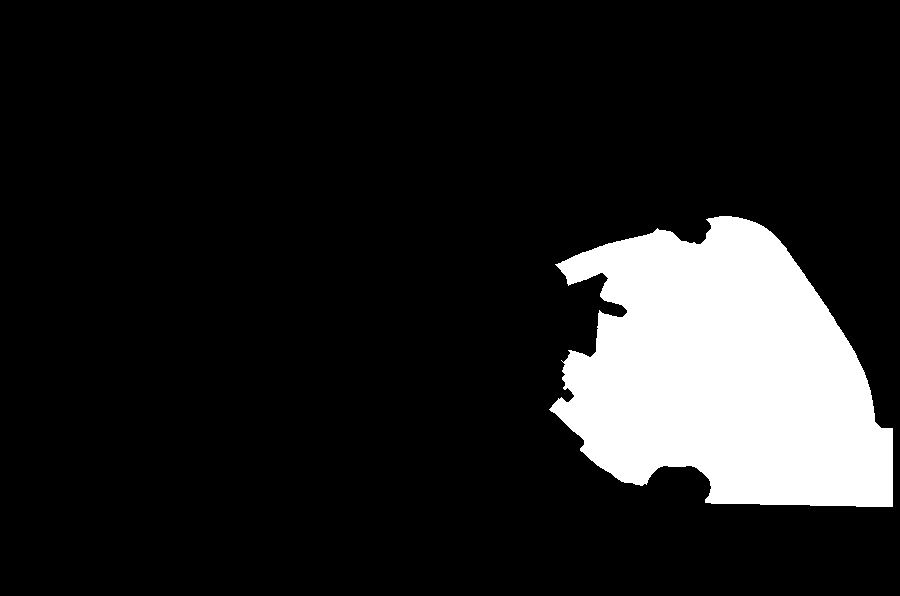
\includegraphics[width=0.95\textwidth]{img/fd2/BackgroundMask.png}
  \caption{}
  % \label{fig:sub2}
\end{subfigure}
\begin{subfigure}{.24\textwidth}
  \centering
  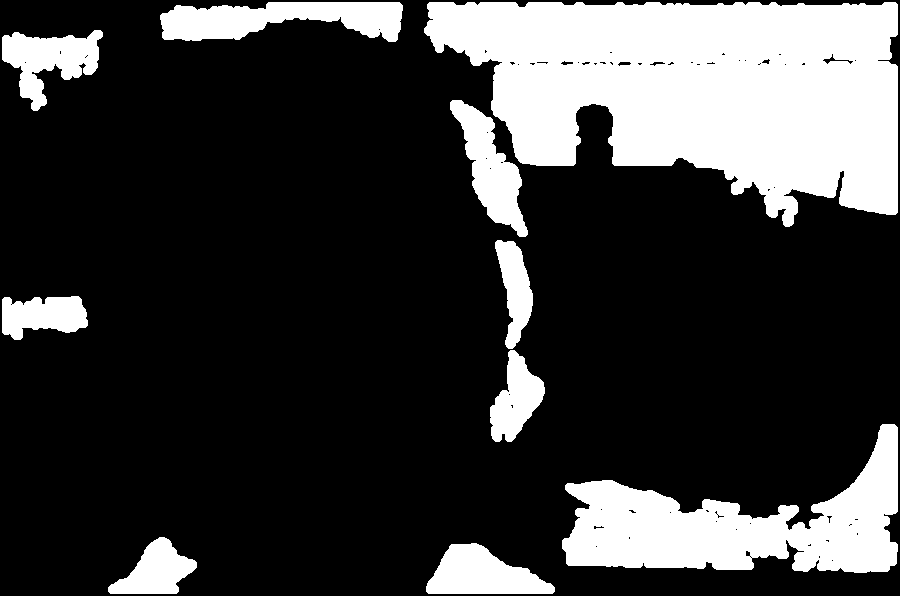
\includegraphics[width=0.95\textwidth]{img/fd/NonFaceMask.png}
  \caption{}
  % \label{fig:sub2}
\end{subfigure}
\begin{subfigure}{.24\textwidth}
  \centering
  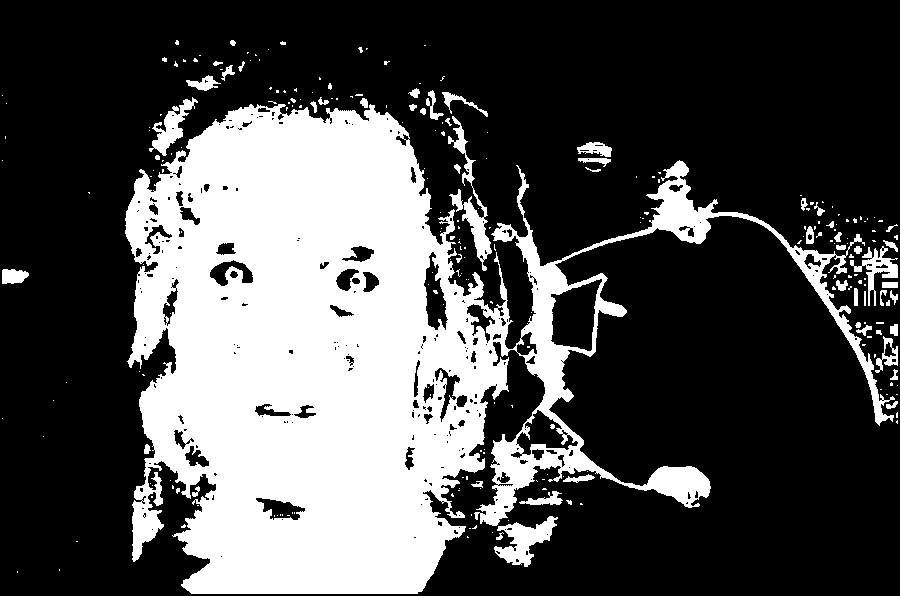
\includegraphics[width=0.95\textwidth]{img/fd/ForegroundMaskAndEstimatedSkinMaskAndNonFaceMask.png}
  \caption{}
  % \label{fig:sub2}
\end{subfigure}


\begin{subfigure}{.24\textwidth}
  \centering
  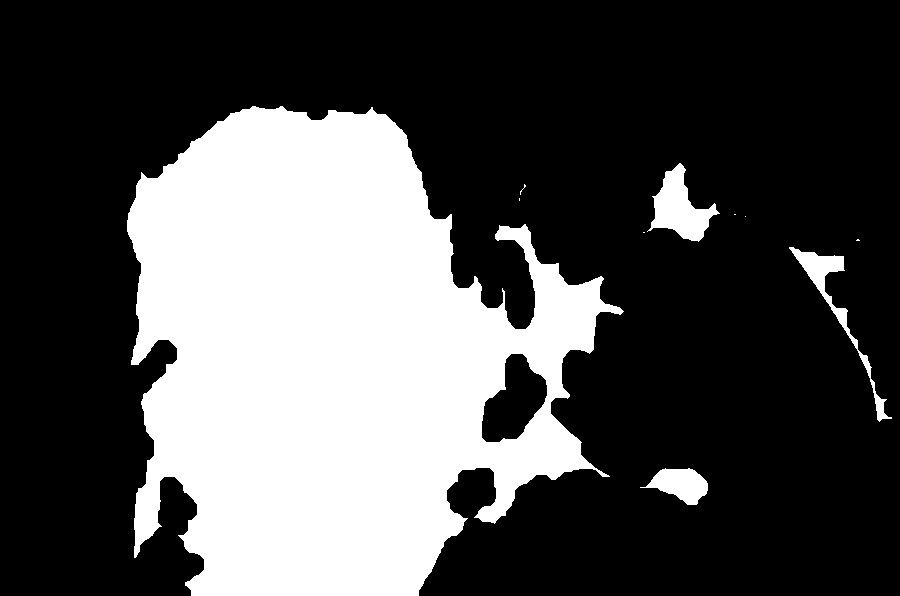
\includegraphics[width=0.95\textwidth]{img/fd/ClosingOnFaceMask.png}
  \caption{}
  % \label{fig:sub2}
\end{subfigure}
\begin{subfigure}{.24\textwidth}
  \centering
  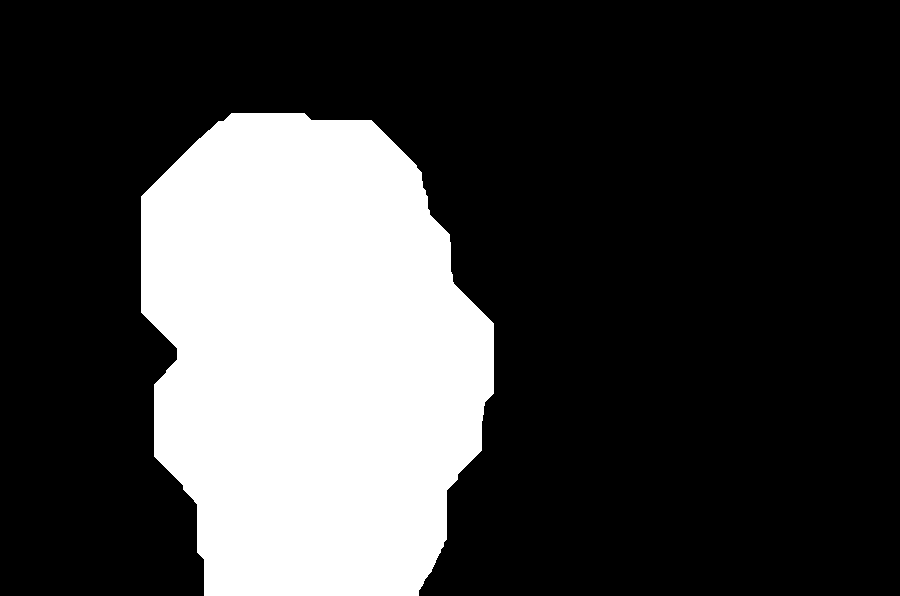
\includegraphics[width=0.95\textwidth]{img/fd/ShrinkFaceMask.png}
  \caption{}
  % \label{fig:sub2}
\end{subfigure}
\begin{subfigure}{.24\textwidth}
  \centering
  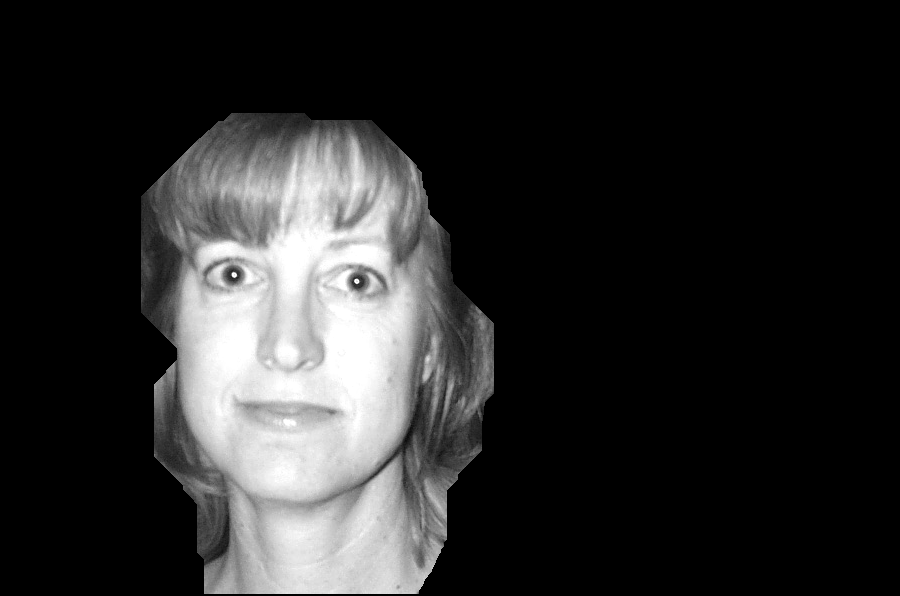
\includegraphics[width=0.95\textwidth]{img/fd/ImadjustGrayFace.png}
  \caption{}
  % \label{fig:sub2}
\end{subfigure}
\begin{subfigure}{.24\textwidth}
  \centering
  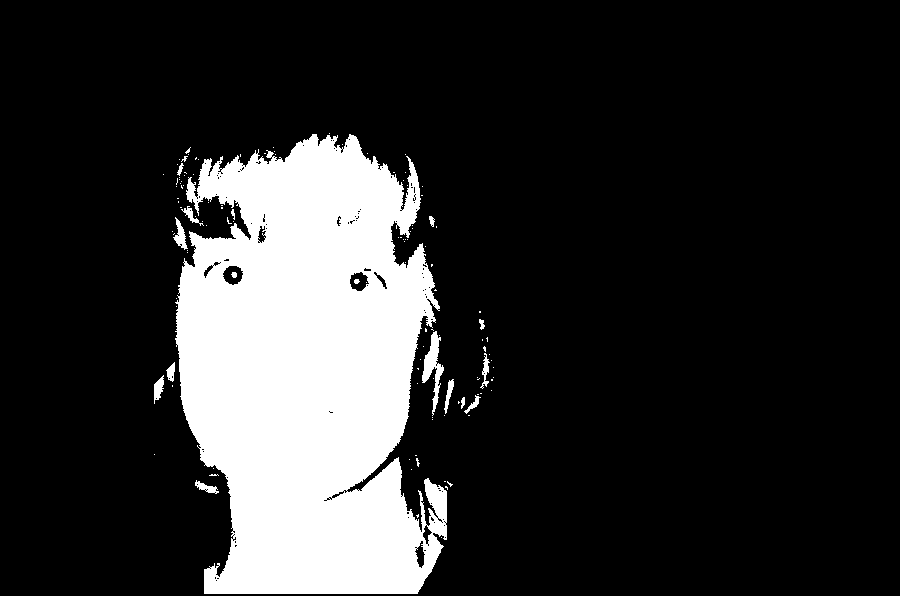
\includegraphics[width=0.95\textwidth]{img/fd/ThresholdGrayFace.png}
  \caption{}
  % \label{fig:sub2}
\end{subfigure}
\begin{subfigure}{.24\textwidth}
  \centering
  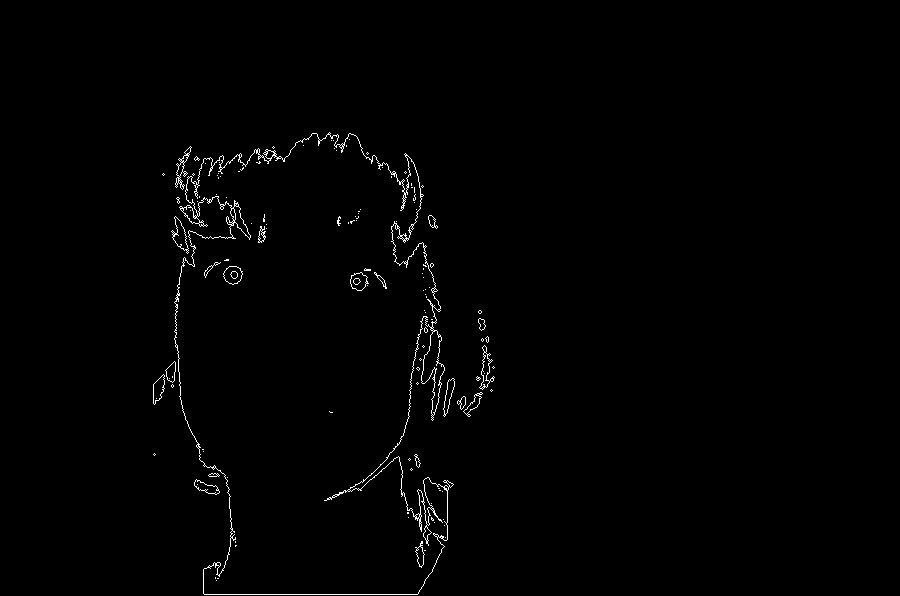
\includegraphics[width=0.95\textwidth]{img/fd/FilteredFaceMask.png}
  \caption{}
  % \label{fig:sub2}
\end{subfigure}
% \begin{subfigure}{.24\textwidth}
%   \centering
%   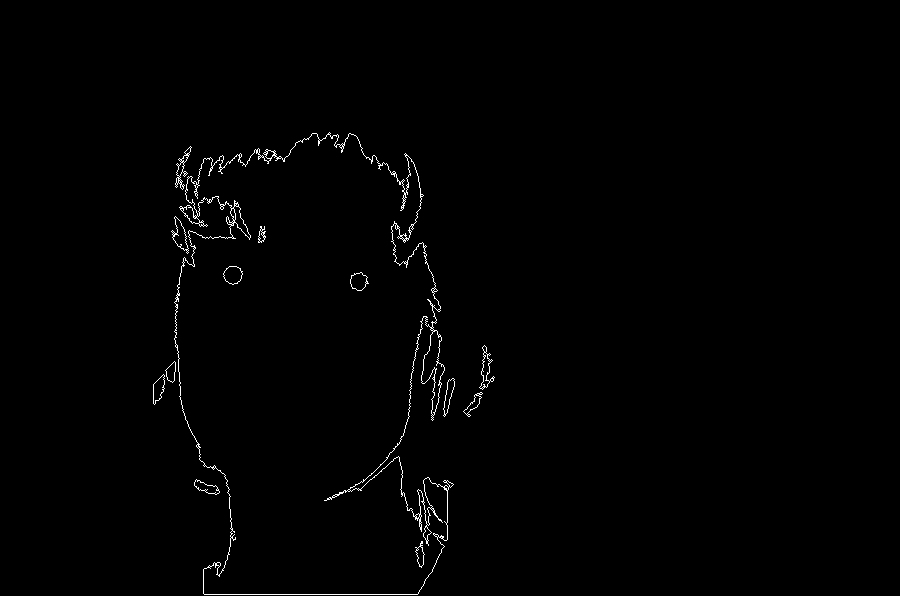
\includegraphics[width=0.95\textwidth]{img/fd/FilteredFaceMask2.png}
%   \caption{}
%   % \label{fig:sub2}
% \end{subfigure}
% \begin{subfigure}{.24\textwidth}
%   \centering
%   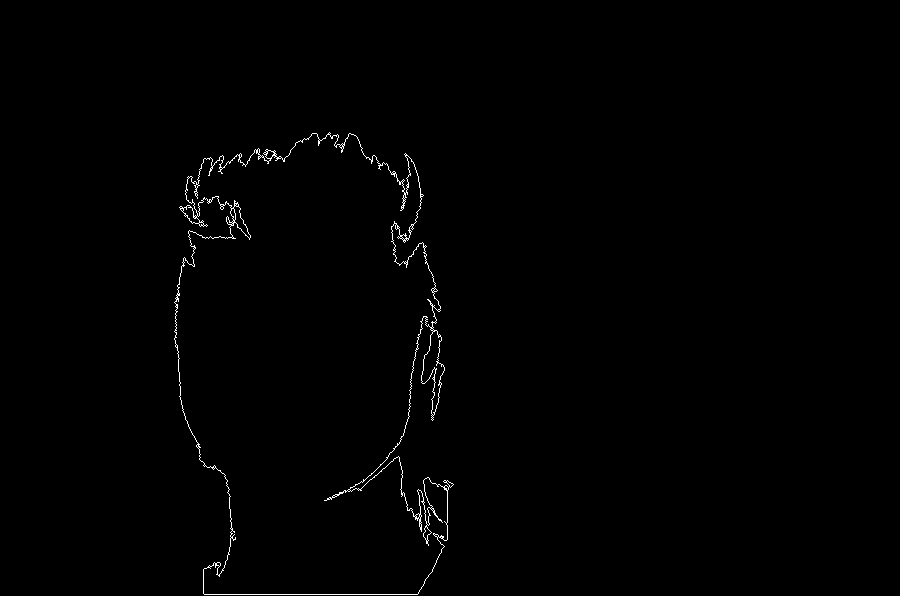
\includegraphics[width=0.95\textwidth]{img/fd/FilteredFaceMask3.png}
%   \caption{}
%   % \label{fig:sub2}
% \end{subfigure}
\begin{subfigure}{.24\textwidth}
  \centering
  
\includegraphics[width=0.95\textwidth]{img/fd/FilteredFaceMask4.png}
  \caption{}
  % \label{fig:sub2}
\end{subfigure}
\begin{subfigure}{.24\textwidth}
  \centering
  
\includegraphics[width=0.95\textwidth]{img/fd/FilteredFaceMask5.png}
  \caption{}
  % \label{fig:sub2}
\end{subfigure}
% \begin{subfigure}{.24\textwidth}
%   \centering
%   
\includegraphics[width=0.95\textwidth]{img/fd/FilteredFaceMask6.png}
%   \caption{}
%   % \label{fig:sub2}
% \end{subfigure}
\begin{subfigure}{.24\textwidth}
  \centering
  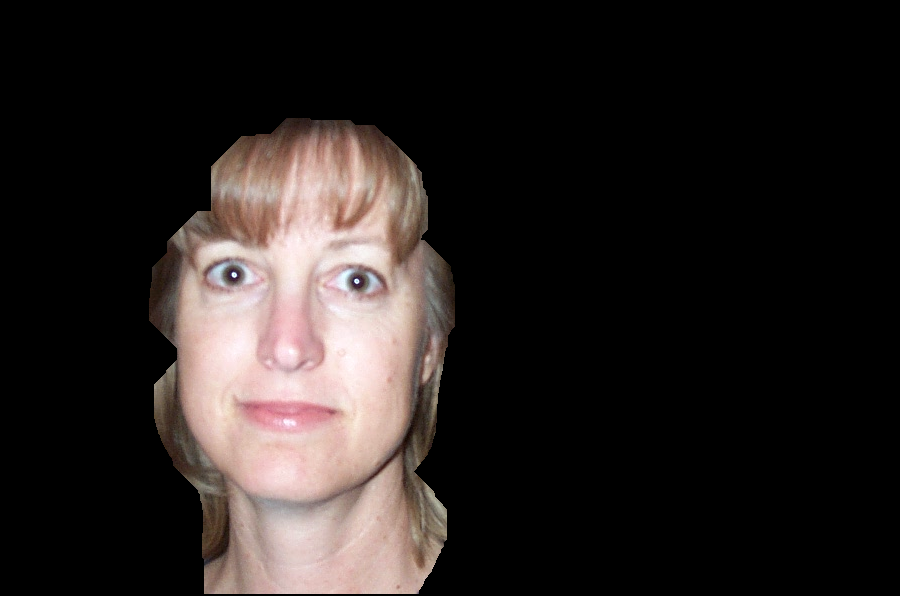
\includegraphics[width=0.95\textwidth]{img/fd/FilteredFaceMask6_Face.png}
  \caption{}
  % \label{fig:sub2}
\end{subfigure}

\caption{Masks \textit{(b-l)} that are generated during the process of deriving the final face \textit{m} from input image \textit{a}.}
\label{fig:faceMasks}
\end{figure}